\chapter{Background}
\label{sec:background}
This chapter provides an overview of the theoretical background of the methods used in this thesis. While the focus of this thesis is the application of machine learning methods in the quantum chemistry context, a basic introduction to compuatational quantum chemistry methods, namely self consistent field (SCF) methods, is provided. 

\section{Self Consistent Field (SCF) Theory}
\label{sec:background_scf}
Quantum chemistry has its roots far before the advent of the computer age. Based on the original theories on quantum mechanics formulated by Schrödinger and Heisenberg, the interest in the accurate description of matter via this new theory was sparked. After the introduction of the wave function by Schrödinger almost century ago Max Born's statistical interpretation enabled a direct calculation of the electrons density. \parencite{ref:schroedinger_1926undulatory} Already a year later Hartree coined a self consistant method to solve the many-electron problem utilizing a mean-field approach. Slater and Fock independently adapted the method by adding the exchange term and consistency with the Pauli exclusion principle. This method was later named Hartree-Fock (HF) method. \parencite{ref:Hartree_1928,ref:slater1930note,ref:fock1930naherungsmethode}. From that point on many advancements have been made in this field. Most prominently density functional therory (DFT), coupled cluster methods (CC), and perturbation theory (MP2) have been developed. Yet the theory behind the HF method is still the basis for many of these methods.

The following introductry overview of the Hartree-Fock method is largely based on the book by Szabo and Ostlund \parencite{ref:szabo_ostlund}. 

\subsection{Ideas behind the Hartree-Fock method}
\label{subsec:background_hf}
The Born Oppenheimer approximations allows for a seperate treatment of the nuclear and electronic problem of a system. This is motivated by the vastly different masses and hence time-scales of nuclei and electron movement. The total wavefunction of a system may be writen as a product state of electronic and nuclear wavefunction (using the convention of small letters for electrons and capital letters for nuclei coordinates):
\begin{equation}
    \Psi_{\text{tot}}(\mathbf{r}_n, \mathbf{R}_m) = \Psi_{\text{elec}}(\mathbf{r}_n; \mathbf{R}_m) \Psi_{\text{nuc}}(\mathbf{R}_m)
\end{equation}
Given our approximation, the total wavefunction can be derived rather easily from the electronic wavefunction via an effective potential for the nuclear motion, given by a solved electronic wavefunction. However, we will focus on the prerequisit of the electronic wavefunction and hence drop the subscript from now on. It depends parametically on the nuclear coordinates and is the solution to the time independent Schrödinger equation:
\begin{equation}
    H \Psi(\mathbf{r}_n; \mathbf{R}_m) = E(\mathbf{R}_m) \Psi(\mathbf{r}_n; \mathbf{R}_m)
\end{equation}
With the electronic energy $E$ being a functional of the electronic wavefunction which will be minimized under ceratin constraints as we'll see later. 
The Hamiltonian operator $H$ reads: 
\begin{equation}
    H = T + V_{\text{ne}} + V_{\text{ee}} = -\frac{1}{2} \sum_{i=1}^N \nabla_i^2 - \sum_{i=1}^N \sum_{A=1}^M \frac{Z_A}{|\mathbf{r}_i - \mathbf{R}_A|} + \sum_{i<j}^N \frac{1}{|\mathbf{r}_i - \mathbf{r}_j|}
\end{equation}
for $N$ electrons and $M$ nuclei in atomic units. Note that we do not include kinetic or repulsion terms for the nuclei as we are only considering the electronic problem. The first term is the kinetic energy operator, the second term describes the interaction of the electrons with the nuclei and the last term describes the electron-electron interaction.\\

Given the Fermionic problem at hand we have to take antisymmetrization into account. Mathematically this can be achieved by writing the wavefunction using a determinant which ensures parity change under exchange of two rows\footnote{Furthermore, if two electrons occupy the same orbital the determinant will vanish}. For $N$ electrons this can be written as:
\begin{equation}
    \Psi(\mathbf{x}_1, \mathbf{x}_2, \ldots, \mathbf{x}_N) = \frac{1}{\sqrt{N!}}
    \begin{vmatrix}
    \chi_1(\mathbf{x}_1) & \chi_2(\mathbf{x}_1) & \cdots & \chi_N(\mathbf{x}_1) \\
    \chi_1(\mathbf{x}_2) & \chi_2(\mathbf{x}_2) & \cdots & \chi_N(\mathbf{x}_2) \\
    \vdots & \vdots & \ddots & \vdots \\
    \chi_1(\mathbf{x}_N) & \chi_2(\mathbf{x}_N) & \cdots & \chi_N(\mathbf{x}_N)
    \end{vmatrix}
\end{equation}
To write down this so called Slater determinant we have introduced the notation $\mathbf{x}_i = (\mathbf{r}_i, \sigma_i)$ with $\sigma_i$ being the spin of electron $i$. The functions $\chi_i$ are called spin orbitals and are a product of spatial and spin functions. 
\begin{equation}
    \chi_i(\mathbf{x}) = \sum_{\mu} C_{i\mu} \chi_\mu(\mathbf{x}) = \sum_{\mu} C_{i\mu} \phi_\mu(\mathbf{r}) \sigma(\sigma) \text{ with } \bra{\chi_i}\ket{\chi_j} = \delta_{ij}
\end{equation}
Using this expansion we reduce the problem to the determination of the coefficients $C_{i\mu}$ for a given set of orthogonal basis functions $\phi_\mu(\mathbf{r})$. For a complete set of basis functions this expansion is exact. However, in practice we have to limit the number of basis functions and hence the size of our Slater determinant to a computationally feasible size. For the subsequent considerations we introduce the shorthand ket for a slater determinant $\ket{\Psi} = \ket{\chi_1, \chi_2, \ldots, \chi_N}$ or $\ket{\Psi} = \ket{1, 2, \ldots, N}$ for the sake of brevity.

%Energy functional
A slater determinants is one simple way of describing the state of a system as a linear combination of basis functions. From that we can derive the energy of the given systems state $E$ using: 
\begin{equation}
    E = \bra{\Psi} H \ket{\Psi}
\end{equation}
For our considerations we will be interested in the ground state of the system. This means we need to find the minimum of our energy functional $E[\Psi]$ and it's corresponding slater determinant $\ket{\Psi}$ which marks our approximation to the ground state wavefunction. This is done via the variational principle which yields an eigenvalue problem: 
\begin{equation}
    \label{eq:hf_eigenval_equation}
    F \ket{\Psi_i} = \varepsilon_i \ket{\Psi_i}
\end{equation}
called the Hartree-Fock equations. Here $\varepsilon_i$ corresponds to the energy of the $i$-th spin-orbital $\ket{\Psi_i}$. The operator $F$ is called the Fock operator and is defined as an effective one electron operator acting on electron $i$:
\begin{equation}
    F(i) = 
    \underbrace{
        -\frac{1}{2} \nabla^2 
        - \sum_{A=1}^M \frac{Z_A}{|\mathbf{r} - \mathbf{R}_A|}
    }_{\text{core Hamiltonian } h(i)}
    + 
    \underbrace{
        \sum_{j\neq i} J_j(i) - K_j(i)
    }_{\text{HF potential }v^{HF}(i)}
\end{equation}
While the core Hamiltonian $h(i)$ contains the well-known kinetic and nuclear attraction terms, the Hartree-Fock potential $v^{HF}(i)$ condenses all electron-electron interaction into a mean-field effect on electron $i$ using the Coulomb and exchange terms:
\begin{subequations}
\begin{align}
    J_j(i)\chi_i(\mathbf{x}_1) &= \left[ \int d\mathbf{x}_2\, \frac{|\chi_j(\mathbf{x}_2)|^2}{r_{12}} \right] \chi_i(\mathbf{x}_1) \\
    K_j(i)\chi_i(\mathbf{x}_1) &= \left[ \int d\mathbf{x}_2\, \frac{\chi_j^*(\mathbf{x}_2)\chi_i(\mathbf{x}_2)}{r_{12}} \right] \chi_j(\mathbf{x}_1)
\end{align}
\end{subequations}
Here, $J_j(i)$ is the Coulomb operator, representing the classical electrostatic repulsion, and $K_j(i)$ is the exchange operator, arising from the antisymmetry of the wavefunction.

While \autoref{eq:hf_eigenval_equation} seems like an ordinary eigenvalue problem, the $\chi$ terms in $J$ and $K$ depend on our slater determinant wavefunction $\ket{\Psi}$. Thus to get the ground state wavefunction, we need the corresponding Fock operator $F$ which in turn depends on the ground state wavefunction. 

%DONE

\subsection{Computational Treatment of the Hartree-Fock Method}
\label{subsec:background_hf_computational}
\TODO{Computational treatment + Überleitung hier her}
The Fock matrix depends on the electron density, which in turn depends on the molecular orbitals, leading to a self-consistent field (SCF) procedure:
\begin{enumerate}
    \item Guess an initial set of molecular orbital coefficients $\mathbf{C}$ (often from a core Hamiltonian or superposition of atomic densities).
    \item Construct the density matrix $\mathbf{P}$ from $\mathbf{C}$.
    \item Build the Fock matrix $\mathbf{F}$ using $\mathbf{P}$.
    \item Solve the generalized eigenvalue problem to obtain new $\mathbf{C}$ and $\mathbf{\varepsilon}$.
    \item Check for convergence of the total energy or density matrix. If not converged, repeat from step 2.
\end{enumerate}

%!Hartree-Fock equations - .... - variational method + energy - matrices used - basis sets - SCF algorithm - kohn-sham equations & DFT - CC / other methods (short) - 
\section{Machine Learning}
\label{sec:background_ml}
%! Intor to ML & Statistical Learning. 
\subsection{Cost Functions}
\label{subsec:background_cost_function}
\TODO{also discuss f-score!!!}

\section{QM9 dataset \parencite{ref:data_qm9}}
\label{sec:qm9}
During selection of a dataset for training two practical considerations dominate. 
\begin{enumerate}
    \item Cost per sample: Time savings through faster convergence are especially relevant for larger systems where the number of SCF iterations are and especially the number of integrals to be calculated are large. Stated differently, it is of very little interest to optimize guessing methods for small systems which converge nearly instantly on conventional hardware. 
    \item Fixed I/O size: Most ML models are constraint to a constant input and output size. 
\end{enumerate}
The QM9 dataset \parencite{ref:article1_qm9,ref:article2_qm9} ticks both of these two boxes. It offers a variety of molecules from as little as 3 constituent atoms up to 29 atoms. Additionally, there are large enough chunks of constitutional isomers to train models on these subsets of same sized matrices. The distribution of molecules by atom count with the predominant constitutional isomers is shown in \autoref{fig:method_qm9_overview}.
%!Figure
% \begin{figure}[H]
%     \centering
%     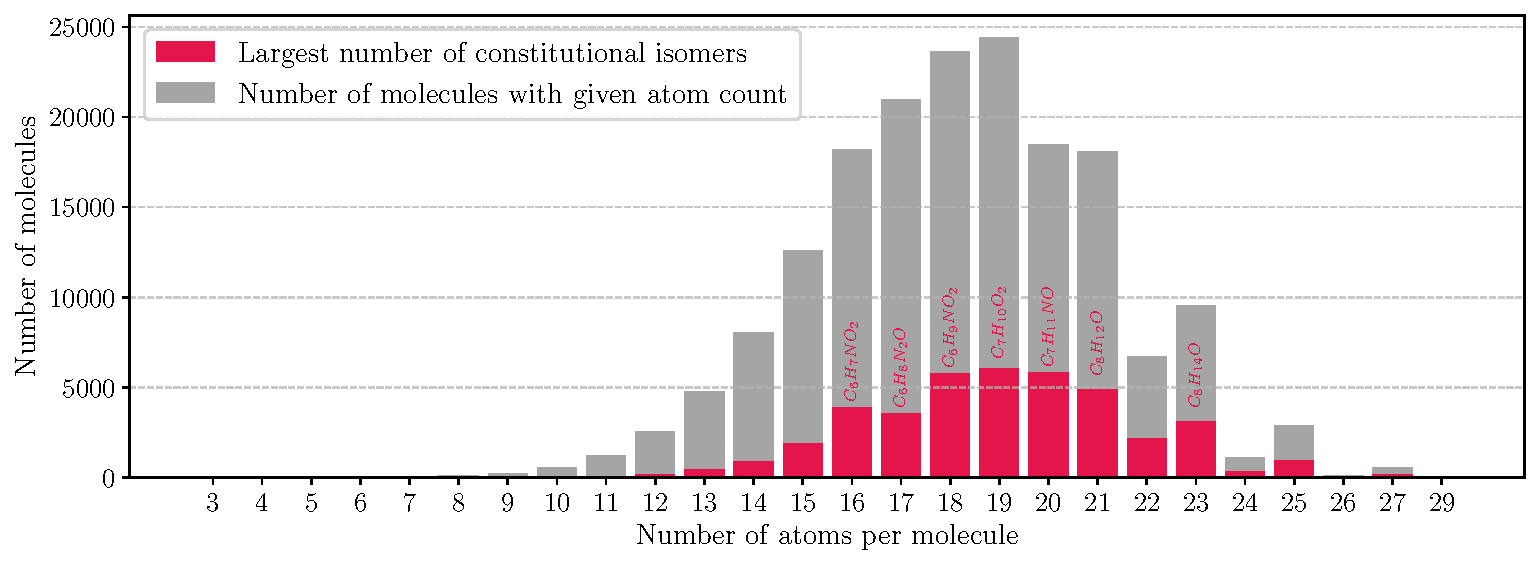
\includegraphics[width=\textwidth]{../fig/qm9_general/qm9_overview_stacked_bar.pdf}
%     \caption[QM9 dataset overview]{Overview of the QM9 dataset. The dataset contains 134k molecules with up to nine heavy - \ch{C} \ch{O} \ch{N} \ch{F} - atoms. Large groups of constitutional isomers are present (largest depicted in red). The properties are calculated using DFT with the B3LYP functional and the 6-31G(2df,p) basis set.}
%     \label{fig:method_qm9_overview}
% \end{figure}
